\subsubsection{抽象化の壁}
データを扱う時に複数の抽象化のレイヤについて考えられる.
分数の例で考えると, 以下の図のようなレイヤが考えられる.
\vskip -0.6cm
\begin{figure}[h]
  \centering
  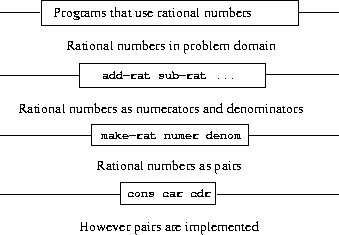
\includegraphics[width=8cm,height=6cm]{imgs/abstraction-barrier.png}
\end{figure}

ここで抽象化のレベルが4つで分かれている. 最も上のレイヤは分数を扱うプログラムが使うもので,
実際分数はどう表現されているかも, どう四則演算が定義されているのかが分からなくても四則演算が
できるレベルである. その下のレイヤでは, 実際四則演算の実装である. そこで分数のセレクタと
コンストラクタを用いるが, その実装に依存しない. その下のレイヤはセレクタとコンストラクタの実装で,
ペアを用いるが今回もその実装に依存しない. 最も下のレイヤはペアの実装である.

そのレイヤ分けの主な利点はプログラムの保守性と柔軟性の向上である.
下のレイヤの実装に依存しないので, データをどう表現するかが変わらない限り,
実装が変わっても影響が受けない.
